%%%%%%%%%%%%%%%%%%%%%%%%%%%%%%%%%%%%
% Slide options
%%%%%%%%%%%%%%%%%%%%%%%%%%%%%%%%%%%%

% Option 1: Slides with solutions

\documentclass[slidestop,compress,mathserif]{beamer}
\newcommand{\soln}[1]{\textit{#1}}
\newcommand{\solnGr}[1]{#1}

% Option 2: Handouts without solutions

%\documentclass[11pt,containsverbatim,handout]{beamer}
%\usepackage{pgfpages}
%\pgfpagesuselayout{4 on 1}[letterpaper,landscape,border shrink=5mm]
%\newcommand{\soln}[1]{ }
%\newcommand{\solnGr}{ }

%%%%%%%%%%%%%%%%%%%%%%%%%%%%%%%%%%%%
% Style
%%%%%%%%%%%%%%%%%%%%%%%%%%%%%%%%%%%%

\def\chp7@path{../../Chp 7}
\input{../../lec_style.tex}


%%%%%%%%%%%%%%%%%%%%%%%%%%%%%%%%%%%%
% Preamble
%%%%%%%%%%%%%%%%%%%%%%%%%%%%%%%%%%%%

\title[Lecture 24]{MA213: Lecture 24}
\subtitle{Module 4: Inference}
\author{OpenIntro Statistics, 4th Edition}
\institute{$\:$ \\ {\footnotesize Based on slides developed by Mine \c{C}etinkaya-Rundel of OpenIntro. \\
The slides may be copied, edited, and/or shared via the \webLink{http://creativecommons.org/licenses/by-sa/3.0/us/}{CC BY-SA license.} \\
Some images may be included under fair use guidelines (educational purposes).}}
\date{}


%%%%%%%%%%%%%%%%%%%%%%%%%%%%%%%%%%%%
% Begin document
%%%%%%%%%%%%%%%%%%%%%%%%%%%%%%%%%%%%

\begin{document}


%%%%%%%%%%%%%%%%%%%%%%%%%%%%%%%%%%%%
% Title page
%%%%%%%%%%%%%%%%%%%%%%%%%%%%%%%%%%%%

{
\addtocounter{framenumber}{-1} 
{\removepagenumbers 
\usebackgroundtemplate{\includegraphics[width=\paperwidth]{../../OpenIntro_Grid_4_3-01.jpg}}
\begin{frame}

\hfill \includegraphics[width=20mm]{../../oiLogo_highres}

\titlepage

\end{frame}
}
}


%%%%%%%%%%%%%%%%%%%%%%%%%%%%%%%%%%%%
% Sections
%%%%%%%%%%%%%%%%%%%%%%%%%%%%%%%%%%%%

%%%%%%%%%%%%%%%%%%%%%%%%%%%%%%%%%%%%

\section{One-sample means with the $t$ distribution}

%%%%%%%%%%%%%%%%%%%%%%%%%%%%%%%%%%%%

\begin{frame}
\frametitle{Friday the 13$^{\text{th}}$}

\dq{Between 1990 - 1992 researchers in the UK collected data on traffic flow, accidents, and hospital admissions on Friday 13$^{\text{th}}$ and the previous Friday, Friday 6$^{\text{th}}$. Below is an excerpt from this data set on traffic flow. We can assume that traffic flow on given day at locations 1 and 2 are independent.}

{\scriptsize
\texttt{
\begin{center}
\begin{tabular}{rllrrrl}
  \hline
 & type & date & 6$^{\text{th}}$ & 13$^{\text{th}}$ & diff & location  \\ 
  \hline
1 & traffic & 1990,  July & 139246 & 138548 & 698 & loc 1 \\
  \rowcolor[gray]{.9}
  2 & traffic & 1990,  July & 134012 & 132908 & 1104 & loc 2 \\
  3 & traffic & 1991,  September & 137055 & 136018 & 1037 & loc 1 \\
  \rowcolor[gray]{.9}
  4 & traffic & 1991,  September & 133732 & 131843 & 1889 & loc 2 \\
  5 & traffic & 1991,  December & 123552 & 121641 & 1911 & loc 1 \\
  \rowcolor[gray]{.9}
  6 & traffic & 1991,  December & 121139 & 118723 & 2416 & loc 2 \\
  7 & traffic & 1992,  March & 128293 & 125532 & 2761 & loc 1 \\
  \rowcolor[gray]{.9}
  8 & traffic & 1992,  March & 124631 & 120249 & 4382 & loc 2 \\
  9 & traffic & 1992,  November & 124609 & 122770 & 1839 & loc 1 \\
  \rowcolor[gray]{.9}
  10 & traffic & 1992,  November & 117584 & 117263 & 321 & loc 2 \\
   \hline
\end{tabular}
\end{center}
}}

\vfill

\rule{2.5cm}{0.25pt} \\
{\tiny Scanlon, T.J., Luben, R.N., Scanlon, F.L., Singleton, N. (1993), ``Is Friday the 13th Bad For Your Health?," BMJ, 307, 1584-1586.}

\end{frame}

%%%%%%%%%%%%%%%%%%%%%%%%%%%%%%%%%%%

\begin{frame}
\frametitle{Friday the 13$^{\text{th}}$}

\begin{itemize}

\item We want to investigate if people's behavior is different on Friday 13$^{\text{th}}$ compared to Friday 6$^{\text{th}}$.

\pause

\item One approach is to compare the traffic flow on these two days.

\pause

\item $H_0:$ Average traffic flow on Friday 6$^{\text{th}}$ and 13$^{\text{th}}$ are equal. \\
$H_A:$ Average traffic flow on Friday 6$^{\text{th}}$ and 13$^{\text{th}}$ are different.

\pause

\end{itemize}

$\:$ \\

\dq{Each case in the data set represents traffic flow recorded at the same location in the same month of the same year: one count from Friday 6$^{\text{th}}$ and the other Friday 13$^{\text{th}}$. Are these two counts independent?}

\soln{\pause No}

\end{frame}

%%%%%%%%%%%%%%%%%%%%%%%%%%%%%%%%%%%

\begin{frame}
\frametitle{Hypotheses}

\pq{What are the hypotheses for testing for a difference between the average traffic flow between Friday 6$^{\text{th}}$ and 13$^{\text{th}}$?}

\begin{enumerate}[(a)]
\item  \mathhl{H_0:} $\mu_{6th} = \mu_{13th}$ \\
\mathhl{H_A:} $\mu_{6th} \ne \mu_{13th}$
\item  \mathhl{H_0:} $p_{6th} = p_{13th}$ \\
\mathhl{H_A:} $p_{6th} \ne p_{13th}$
\solnMult{ \mathhl{H_0:} $\mu_{diff} = 0$ \\
\mathhl{H_A:} $\mu_{diff} \ne 0$ }
\item  \mathhl{H_0:} $\bar{x}_{diff} = 0$ \\
\mathhl{H_A:} $\bar{x}_{diff} = 0$
\end{enumerate}

\end{frame}

%%%%%%%%%%%%%%%%%%%%%%%%%%%%%%%%%%%

\begin{frame}
\frametitle{Conditions}

\begin{itemize}

\item \hl{Independence:} We are told to assume that cases (rows) are independent.

\pause

\item \hl{Sample size / skew:} $\:$ \\

\pause

\twocol{0.75}{0.35}
{
{\tiny
\begin{itemize}

\item The sample distribution does not appear to be extremely skewed, but it's very difficult to assess with such a small sample size. We might want to think about whether we would expect the population distribution to be skewed or not -- probably not, it should be equally likely to have days with lower than average traffic and higher than average traffic.

\item We do not know $\sigma$ and $n$ is too small to assume $s$ is a reliable estimate for $\sigma$.
\end{itemize}
}
}
{
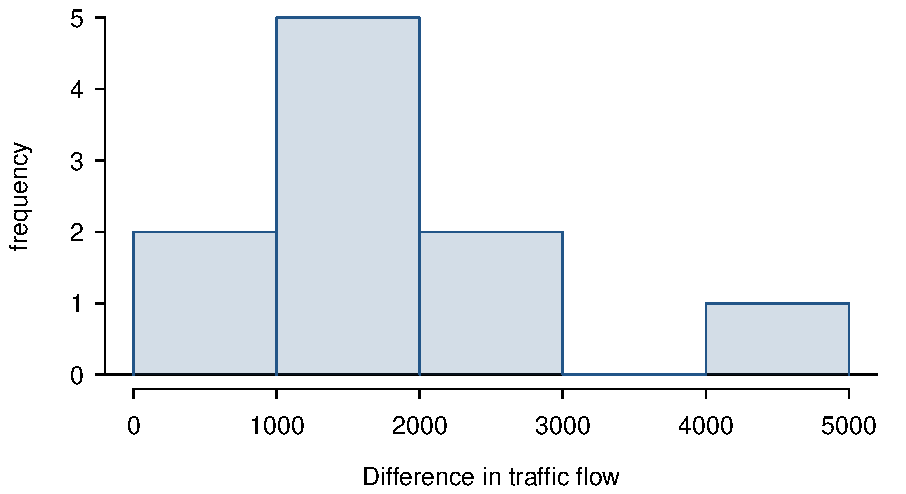
\includegraphics[width=\textwidth]{\chp7@path/7-1_one_t/figures/friday/trafficHist}
}

\end{itemize}

$\:$ \\

\pause

\dq{So what do we do when the sample size is small?}

\end{frame}

%%%%%%%%%%%%%%%%%%%%%%%%%%%%%%%%%%%

\section{Edfinity Quiz: Intuition check, and what tools do we have for this problem?}

%%%%%%%%%%%%%%%%%%%%%%%%%%%%%%%%%%%

\section{R Demonstration: Try something and see what happens}

%%%%%%%%%%%%%%%%%%%%%%%%%%%%%%%%%%%

\begin{frame}
\frametitle{Review: what purpose does a large sample serve?}

As long as observations are independent, and the population distribution is not extremely skewed, a large sample would ensure that...

\begin{itemize}

\item the sampling distribution of the mean is nearly normal

\item the estimate of the standard error, as $\frac{s}{\sqrt{n}}$, is reliable

\end{itemize}

\end{frame}

%%%%%%%%%%%%%%%%%%%%%%%%%%%%%%%%%%%

\subsection{The normality condition}

%%%%%%%%%%%%%%%%%%%%%%%%%%%%%%%%%%%

\begin{frame}
\frametitle{The normality condition}

\begin{itemize}

\item The CLT, which states that sampling distributions will be nearly normal, holds true for \orange{any} sample size as long as the population distribution is nearly normal.

\pause

\item While this is a helpful special case, it's inherently difficult to verify normality in small data sets.

\pause

\item We should exercise caution when verifying the normality condition for small samples. It is important to not only examine the data but also think about where the data come from. 
\begin{itemize}
\item For example, ask: would I expect this distribution to be symmetric, and am I confident that outliers are rare?
\end{itemize}

\end{itemize}

\end{frame}

%%%%%%%%%%%%%%%%%%%%%%%%%%%%%%%%%%%

\subsection{Introducing the $t$ distribution}

%%%%%%%%%%%%%%%%%%%%%%%%%%%%%%%%%%%

\begin{frame}
\frametitle{The $t$ distribution}

\begin{itemize}

\item When the population standard deviation is unknown (almost always), the uncertainty of the standard error estimate is addressed by using a new distribution: the \hl{$t$ distribution}.

\pause

\item This distribution also has a bell shape, but its tails are \hl{thicker} than the normal model's.

\pause

\item Therefore observations are more likely to fall beyond two SDs from the mean than under the normal distribution.

\pause

\item Extra thick tails are helpful for resolving our problem with a less reliable estimate the standard error (since $n$ is small)

\end{itemize}

\begin{center}
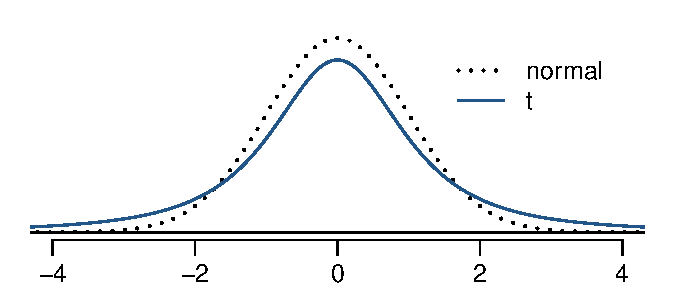
\includegraphics[width=0.5\textwidth]{\chp7@path/7-1_one_t/figures/tDistCompareToNormalDist/tDistCompareToNormalDist}
\end{center}

\end{frame}

%%%%%%%%%%%%%%%%%%%%%%%%%%%%%%%%%%%

\begin{frame}
\frametitle{The $t$ distribution (cont.)}

\begin{itemize}

\item Always centered at zero, like the standard normal ($z$) distribution.

\item Has a single parameter: \hl{degrees of freedom} (\mathhl{df}).

\end{itemize}

\begin{center}
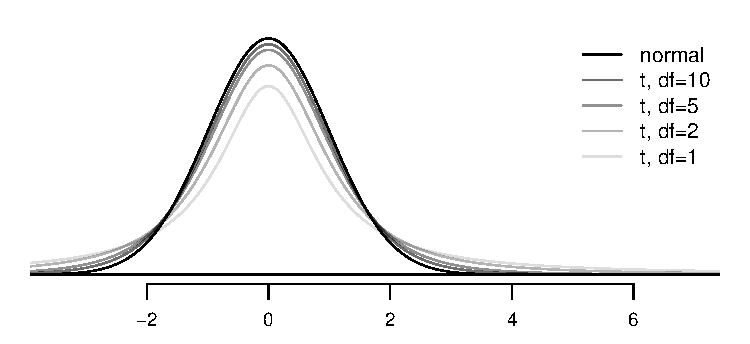
\includegraphics[width=0.8\textwidth]{\chp7@path/7-1_one_t/figures/tDistConvergeToNormalDist/tDistConvergeToNormalDist}
\end{center}

\pause

\dq{What happens to shape of the $t$ distribution as $df$ increases?}

\soln{\pause Approaches normal.}

\end{frame}

%%%%%%%%%%%%%%%%%%%%%%%%%%%%%%%%%%%

\subsection{Evaluating hypotheses using the $t$ distribution}

%%%%%%%%%%%%%%%%%%%%%%%%%%%%%%%%%%%

\section{R Demonstration: Try with $t$ distribution}

%%%%%%%%%%%%%%%%%%%%%%%%%%%%%%%%%%%

\begin{frame}
\frametitle{Back to Friday the 13$^{\text{th}}$}

\vspace{-1cm}

{\footnotesize
\texttt{
\begin{center}
\begin{tabular}{rllrr || r || l}
  \hline
 & type & date & 6$^{\text{th}}$ & 13$^{\text{th}}$ & diff & location  \\ 
  \hline
1 & traffic & 1990,  July & 139246 & 138548 & 698 & loc 1 \\
  \rowcolor[gray]{.9}
  2 & traffic & 1990,  July & 134012 & 132908 & 1104 & loc 2 \\
  3 & traffic & 1991,  September & 137055 & 136018 & 1037 & loc 1 \\
  \rowcolor[gray]{.9}
  4 & traffic & 1991,  September & 133732 & 131843 & 1889 & loc 2 \\
  5 & traffic & 1991,  December & 123552 & 121641 & 1911 & loc 1 \\
  \rowcolor[gray]{.9}
  6 & traffic & 1991,  December & 121139 & 118723 & 2416 & loc 2 \\
  7 & traffic & 1992,  March & 128293 & 125532 & 2761 & loc 1 \\
  \rowcolor[gray]{.9}
  8 & traffic & 1992,  March & 124631 & 120249 & 4382 & loc 2 \\
  9 & traffic & 1992,  November & 124609 & 122770 & 1839 & loc 1 \\
  \rowcolor[gray]{.9}
  10 & traffic & 1992,  November & 117584 & 117263 & 321 & loc 2 \\
   \hline
\end{tabular}
\end{center}
}}

\begin{align*}
\hspace{6cm} &\orange{$\bar{x}_{diff} = 1836$} \\
& \orange{$s_{diff} = 1176$} \\
& \orange{$n = 10$} 
\end{align*}
 
\end{frame}

%%%%%%%%%%%%%%%%%%%%%%%%%%%%%%%%%%%

\begin{frame}
\frametitle{Finding the test statistic}

\formula{Test statistic for inference on a small sample mean}
{The test statistic for inference on a small sample ($n < 50$) mean is the $T$ statistic with $df = n - 1$.
\[ T_{df} = \frac{\text{point estimate} - \text{null value}}{SE} \]}

\pause

\vspace{-0.5cm}

\hl{in context...}
\begin{eqnarray*}
point~estimate &=& \bar{x}_{diff} = 1836 \\
\pause
SE &=& \frac{s_{diff}}{\sqrt{n}} = \frac{1176}{\sqrt{10}} = 372 \\
\pause
T &=& \frac{1836 - 0}{372} = 4.94 \\
\pause
df &=& 10 - 1 = 9
\end{eqnarray*}

\vspace{-0.25cm}

\Note{Null value is 0 because in the null hypothesis we set $\mu_{diff} = 0$.}

\end{frame}

%%%%%%%%%%%%%%%%%%%%%%%%%%%%%%%%%%%

\begin{frame}[fragile]
\frametitle{Finding the p-value}

\begin{itemize}

\item The p-value is, once again, calculated as the area tail area under the $t$ distribution.

\pause

\item Using R:
\begin{verbatim}
> 2 * pt(4.94, df = 9, lower.tail = FALSE)

[1] 0.0008022394
\end{verbatim}

\pause

\item Using a web app:

\href{https://gallery.shinyapps.io/dist_calc/}{\textcolor{oiB}{https://gallery.shinyapps.io/dist\_calc/}}

\pause

\item Or when these aren't available, we can use a $t$-table.

\end{itemize}

\end{frame}

%%%%%%%%%%%%%%%%%%%%%%%%%%%%%%%%%%%


\begin{frame}
\frametitle{Conclusion of the test}

\dq{What is the conclusion of this hypothesis test?}

\pause

Since the p-value is quite low, we conclude that the data provide strong evidence of a difference between traffic flow on Friday 6$^{\text{th}}$ and 13$^{\text{th}}$.

\end{frame}

%%%%%%%%%%%%%%%%%%%%%%%%%%%%%%%%%%%%

\subsection{Constructing confidence intervals using the $t$ distribution}

%%%%%%%%%%%%%%%%%%%%%%%%%%%%%%%%%%%

\begin{frame}
\frametitle{What is the difference?}

\begin{itemize}

\item We concluded that there is a difference in the traffic flow between Friday 6$^{\text{th}}$ and 13$^{\text{th}}$.

\pause

\item But it would be more interesting to find out what exactly this difference is.

\pause

\item We can use a confidence interval to estimate this difference.

\end{itemize}

\end{frame}

%%%%%%%%%%%%%%%%%%%%%%%%%%%%%%%%%%%

\section{Edfinity Quiz: What is the difference? Try for yourself!}

%%%%%%%%%%%%%%%%%%%%%%%%%%%%%%%%%%%

\begin{frame}
\frametitle{Confidence interval for a small sample mean}

\begin{itemize}

\item Confidence intervals are always of the form
\[ \text{point estimate} \pm {ME} \]

\pause

\item ME is always calculated as the product of a critical value and SE.

\pause

\item Since small sample means follow a $t$ distribution (and not a $z$ distribution), the critical value is a $t^\star$ (as opposed to a $z^\star$).
\[ \text{point estimate} \pm t^{\star} \times SE \]

\end{itemize}

\end{frame}

%%%%%%%%%%%%%%%%%%%%%%%%%%%%%%%%%%%

\begin{frame}[fragile]
\frametitle{Finding the critical $t$ ($t^\star$)}


Using R:
\begin{verbatim}

> qt(p = 0.975, df = 9)

[1] 2.262157

\end{verbatim}

\end{frame}

%%%%%%%%%%%%%%%%%%%%%%%%%%%%%%%%%%%

\begin{frame}
\frametitle{Constructing a CI for a small sample mean}

\pq{Which of the following is the correct calculation of a 95\% confidence interval for the difference between the traffic flow between Friday 6$^{\text{th}}$ and 13$^{\text{th}}$?}
\[ \bar{x}_{diff} = 1836 \qquad s_{diff} = 1176 \qquad n = 10 \qquad SE = 372 \]

\twocol{0.35}{0.65}
{
\begin{enumerate}[(a)]

\item $1836 \pm 1.96 \times 372$

\solnMult{ $1836 \pm 2.26 \times 372$}

\item $1836 \pm -2.26 \times 372$

\item $1836 \pm 2.26 \times 1176$

\end{enumerate}
}
{
\soln{\only<2>{\orange{$\rightarrow$ (995, 2677)}}}
\vspace{0.25cm}
}

\end{frame}

%%%%%%%%%%%%%%%%%%%%%%%%%%%%%%%%%%%

\begin{frame}
\frametitle{Interpreting the CI}

\pq{Which of the following is the \orange{best} interpretation for the confidence interval we just calculated?
\[ \mu_{diff: 6th - 13th} = (995, 2677) \]
}

We are 95\% confident that ...

\begin{enumerate}[(a)]

\item the difference between the average number of cars on the road on Friday 6$^{\text{th}}$ and 13$^{\text{th}}$ is between 995 and 2,677.

\item on Friday 6$^{\text{th}}$ there are 995 to 2,677 fewer cars on the road than on the Friday 13$^{\text{th}}$, on average.

\item on Friday 6$^{\text{th}}$ there are 995 fewer to 2,677 more cars on the road than on the Friday 13$^{\text{th}}$, on average.

\solnMult{ on Friday 13$^{\text{th}}$ there are 995 to 2,677 fewer cars on the road than on the Friday 6$^{\text{th}}$, on average.}

\end{enumerate}

\end{frame}

%%%%%%%%%%%%%%%%%%%%%%%%%%%%%%%%%%%

\subsection{Synthesis}

%%%%%%%%%%%%%%%%%%%%%%%%%%%%%%%%%%%

\begin{frame}
\frametitle{Synthesis}

\dq{Does the conclusion from the hypothesis test agree with the findings of the confidence interval?}

$\:$ \\

\soln{\only<2->{Yes, the hypothesis test found a significant difference, and the CI does not contain the null value of 0.}}

$\:$ \\

\dq{Do you think the findings of this study suggests that people believe Friday 13$^{\text{th}}$ is   a day of bad luck?}

$\:$ \\

\soln{\only<3>{No, this is an observational study. We have just observed a significant difference between the number of cars on the road on these two days. We have not tested for people's beliefs.}}

\end{frame}

%%%%%%%%%%%%%%%%%%%%%%%%%%%%%%%%%%%

\begin{frame}
\frametitle{Recap: Inference using the $t$-distribution}

\begin{itemize}

\item If $\sigma$ is unknown, use the $t$-distribution with $SE = \frac{s}{\sqrt{n}}$.

\pause

\item Conditions: 
\begin{itemize}
\item independence of observations (often verified by random sample, and if sampling w/o replacement, $n < $ 10\% of population)
\item no extreme skew
\end{itemize}

\pause

\item Hypothesis testing: 
\[ T_{df} = \frac{\text{point estimate} - \text{null value}}{SE}\text{, where }df = n - 1 \]

\pause

\item Confidence interval: $\text{point estimate} \pm t_{df}^\star \times SE$

\end{itemize}

\pause

\vspace{-0.25cm}

\Note{The example we used was for paired means (difference between dependent groups). We took the difference between the observations and used only these differences (one sample) in our analysis, therefore the mechanics are the same as when we are working with just one sample.}

\end{frame}

%%%%%%%%%%%%%%%%%%%%%%%%%%%%%%%%%%%

%%%%%%%%%%%%%%%%%%%%%%%%%%%%%%%%%%%%
% End document
%%%%%%%%%%%%%%%%%%%%%%%%%%%%%%%%%%%%

\end{document}